\chapter{Evaluation}
\label{ch:evaluation}

% Render this chapter's tables and figures inline (where written) rather than letting them float.
\floatplacement{table}{H}
\floatplacement{figure}{H}

This chapter evaluates the coupled adaptive system of~\cref{ch:implementation} against the attacks specified in~\cref{sec:axt-scope}. It is organised around the three research questions of this thesis, relating to: the attack surface the coupling exposes (RQ1), poisoning attacks on the base learner through the composition channel (RQ2), and evasion attacks on the detector through the trigger channel (RQ3). Each is presented as a hypothesis, the results, and a discussion.~\cref{sec:eval-settings} fixes the elements common to every experiment; experimental settings that vary between them are stated in a \textit{Setup} note at the head of each section.

\section{Experimental Settings}
\label{sec:eval-settings}
The victim throughout is the full coupled system, \textsc{AdaptiveDAdaptiveM} of~\cref{sec:impl-configs}, in which both the detector $\mathcal{D}$ and the base learner $\mathcal{M}$ are rebuilt at each concept-discovery event. Two reduced configurations serve as references where an ablation requires them: \textsc{StaticDStaticM}, which never adapts and fixes the no-adaptation floor, and \textsc{StaticDAdaptiveM}, in which the encoder is frozen but $\mathcal{M}$ still rebuilds.

The stream is the Monday--Friday CICIDS2017 trace (Engelen-corrected,~\cref{sec:impl-data}) replayed in temporal order; \texttt{DoS} and \texttt{PortScan} are held out as the two novel classes that arrive mid-week, so that genuine drift is present in every run. The adversary acts through the injection model of~\cref{sec:impl-injection}. Every detector is calibrated by the rule of~\cref{sec:impl-calibration}, but the resulting threshold values depend on the detector's training set and are therefore stated per experiment. We report $F_1$ measures against a fixed novel-class-aware benchmark and per-class false-negative rate (FNR) alongside it.

\section{Baseline Behaviour Under Genuine Drift}
\label{sec:eval-baseline}
\textit{Setup.} The \textsc{AdaptiveDAdaptiveM} victim is trained on the full known-class pool ($T_{drift} = 1.34$, $T = 37.84$), run on the unpoisoned stream and averaged over three seeds.

Before introducing an adversary we confirm that, on an unpoisoned stream, the coupled system adapts to the genuine drift. It discovers \texttt{DoS} as it arrives mid-week (registering it as a new concept and rebuilding once) and recovers to a Friday $F_1$ of $0.71$ against the no-adaptation floor of $0.207$ (\cref{tab:baseline-adaptation}). It does \emph{not}, however, discover \texttt{PortScan}: that class embeds too close to a known prototype to be flagged as drift (\cref{sec:eval-rq2}), so the system adapts to only one of the two novel classes. This run is the reference point for every attack that follows.

\cref{tab:baseline-adaptation} makes this concrete by comparing the full system (\textsc{AdaptiveDAdaptiveM}) to the static floor (\textsc{StaticDStaticM}, where $\mathcal{M}$ never updates), on aggregate $F_1$ and per-class false-negative rate. Both sit at the floor on Monday and Tuesday; once \texttt{DoS} is discovered during Wednesday, the full system's aggregate $F_1$ climbs from $0.207$ to $0.710$ and its \texttt{DoS} false-negative rate falls from $0.881$ to $0.008$, while the static floor stays put all week. However, the \texttt{PortScan} false-negative rate barely moves from the floor's $0.999$ to $0.983$. This is because the system never discovers that class. We report per-class rates throughout for exactly this reason: aggregate $F_1$ alone would hide a whole novel class going undetected.

\begin{table}
\caption{Baseline (no attack) per-day metrics for the static reference and the full system. $F_1$ is measured against a fixed novel-class-aware benchmark and false-negative rate is measured for \texttt{DoS} and \texttt{PortScan}, whose novel instances arrive on Wednesday and Friday respectively.}
\label{tab:baseline-adaptation}
\centering
\begin{tabular}{lcccccc}
\toprule
 & \multicolumn{3}{c}{\textsc{StaticDStaticM}} & \multicolumn{3}{c}{\textsc{AdaptiveDAdaptiveM}} \\
\cmidrule(lr){2-4}\cmidrule(lr){5-7}
Day & $F_1$ & FNR(\texttt{DoS}) & FNR(\texttt{PortScan}) & $F_1$ & FNR(\texttt{DoS}) & FNR(\texttt{PortScan}) \\
\midrule
Mon & 0.207 & 0.881 & 0.999 & 0.207 & 0.881 & 0.999 \\
Tue & 0.207 & 0.881 & 0.999 & 0.207 & 0.881 & 0.999 \\
Wed & 0.207 & 0.881 & 0.999 & 0.346 & 0.640 & 0.995 \\
Thu & 0.207 & 0.881 & 0.999 & 0.710 & 0.008 & 0.983 \\
Fri & 0.207 & 0.881 & 0.999 & 0.710 & 0.008 & 0.983 \\
\bottomrule
\end{tabular}
\end{table}


\clearpage

\section{RQ1 -- The Attack Surfaces of the Coupling}
\label{sec:eval-rq1}
\textit{Hypothesis.} The trigger-dependent coupling exposes attack surfaces that a continuously-updated learner does not. Namely, a trigger channel that decides when rebuilds occur, and a composition channel that decides what data rebuilds use.

The baseline run is itself the evidence. Because $\mathcal{M}$ changes only when the predicate fires (\cref{tab:baseline-adaptation}), the trigger gates all adaptation. This means an adversary who controls whether the predicate fires controls whether $\mathcal{M}$ ever learns the emerging class, and an adversary who controls the buffer at a firing event controls what it learns. A continuously-updated learner offers no such discrete gate; its decision boundary is a moving target that dilutes any single injection. The remainder of the chapter exploits exactly these two surfaces: RQ2 attacks the composition channel and RQ3 the trigger channel. Both are properties of the coupling and both are invisible to a detector-only evaluation.
\clearpage

\section{RQ2 -- The Composition Channel: Poisoning and Backdooring the Base Learner}
\label{sec:eval-rq2}
\textit{Hypothesis.} The composition channel (the data a firing event retrains on) lets the adversary corrupt $\mathcal{M}$ through its retraining set.

\textit{Setup.} The victim is the full-data \textsc{AdaptiveDAdaptiveM} ($T_{drift} = 1.34$, $T = 37.84$). The adversary acts only through the benign-labelled injection of~\cref{sec:impl-injection}; its rate, schedule, and feature perturbations vary by experiment and are stated where each is introduced. All results average three seeds.

Contrary to the hypothesis, a base learner retrained from scratch to convergence \emph{resists} this poisoning. Sweeping a benign-labelled injection of novel \texttt{DoS} flows over $p \in \{0, 5, \dots, 35\}\%$ and riding the genuine mid-week drift event, so that the mislabelled flows are placed into $\mathcal{M}$'s retraining set, leaves the \texttt{DoS} false-negative rate essentially at its clean value across the low and mid budgets ($0.019$ at $p = 0$, $0.014$ at $5\%$, $0.033$ at $20\%$ --~\cref{tab:attack-fri-summary}). The mislabelled flows are a down-weighted minority in a set dominated by correctly-labelled exemplars, so the rebuilt $\mathcal{M}$ still classifies \texttt{DoS} correctly. Persistence does not help: a \emph{durable} variant that injects only around the fire and then stops, lodging its payload in the never-evict exemplar memory, is absorbed just the same. The large per-class damage that a single under-trained rebuild would expose is therefore an artefact of the retraining recipe, not of the coupling; an encoder-freeze ablation (\textsc{StaticDAdaptiveM}) confirms there is no representation-level poisoning to relocate, the frozen-encoder false-negative rate being no lower than the adapting one.

\begin{table}
\caption{Friday end-of-stream attack effect on the full coupled adaptive IDS (\textsc{AdaptiveDAdaptiveM}). Values are mean $\pm$ std across three seeds.}
\label{tab:attack-fri-summary}
\resizebox{\textwidth}{!}{
\begin{tabular}{llcccl}
\toprule
 & Poison \% & Fri $F_1$ & Fri FNR(\texttt{DoS}) & Fri FNR(\texttt{PS}) & Retrains \\
System &  &  &  &  & \\
\midrule
\textsc{StaticDStaticM} & ref & 0.207 $\pm$ 0.000 & 0.881 $\pm$ 0.000 & 0.999 $\pm$ 0.000 & 0 \\
\textsc{AdaptiveDAdaptiveM} & 0 & 0.710 $\pm$ 0.000 & 0.008 $\pm$ 0.000 & 0.983 $\pm$ 0.000 & 1 \\
\textsc{AdaptiveDAdaptiveM} & 5 & 0.726 $\pm$ 0.034 & 0.014 $\pm$ 0.006 & 0.903 $\pm$ 0.137 & 1.3$\pm$0.5 \\
\textsc{AdaptiveDAdaptiveM} & 15 & 0.820 $\pm$ 0.053 & 0.030 $\pm$ 0.003 & 0.529 $\pm$ 0.205 & 2.0$\pm$0.0 \\
\textsc{AdaptiveDAdaptiveM} & 20 & 0.821 $\pm$ 0.053 & 0.033 $\pm$ 0.002 & 0.508 $\pm$ 0.175 & 2.0$\pm$0.0 \\
\textsc{AdaptiveDAdaptiveM} & 25 & 0.207 $\pm$ 0.000 & 0.881 $\pm$ 0.000 & 0.999 $\pm$ 0.000 & 0.0$\pm$0.0 \\
\textsc{AdaptiveDAdaptiveM} & 30 & 0.680 $\pm$ 0.006 & 0.055 $\pm$ 0.011 & 1.000 $\pm$ 0.000 & 1.0$\pm$0.0 \\
\textsc{AdaptiveDAdaptiveM} & 35 & 0.702 $\pm$ 0.001 & 0.006 $\pm$ 0.001 & 1.000 $\pm$ 0.000 & 1.0$\pm$0.0 \\
\bottomrule
\end{tabular}
}
\end{table}

So, the boundary cannot be moved against the genuine class, but it can be circumvented. The channel admits a backdoor, which succeeds precisely because it does not contend with the clean decision boundary. Rather than just mislabelling \texttt{DoS} as benign, the adversary also stamps them with a small feature-space trigger, teaching $\mathcal{M}$ that ``\texttt{DoS}-features $+$ trigger $\Rightarrow$ benign''. The trigger is inert on an un-poisoned learner -- it moves the \texttt{DoS} false-negative rate from $0.012$ to $0.014$ -- but after the backdoor is planted a \emph{triggered} \texttt{DoS} flow evades $\mathcal{M}$ with false-negative rate $0.69$, while \emph{clean} \texttt{DoS} is still caught (with false-negative rate $0.03$). The backdoor is also durable: the adversary injects only around the genuine mid-week fire and then stops, yet the backdoor persists regardless of any further retrains. This is because of all the harvested concept exemplars that carry the trigger being replayed into every subsequent rebuild -- the never-evict exemplar memory (\cref{sec:impl-retrain}) turned against the system. An ablation that disables this memory isolates its role (\cref{tab:rq2-backdoor}). With the harvested exemplars retained (accum=500) the triggered false-negative rate stays consistently high ($0.687 \pm 0.096$), whereas disabling them (accum=0) leaves the same mean ($0.679$) but makes persistence highly seed-dependent ($\pm 0.454$). Therefore, we can confirm that the never-evict memory is what makes the backdoor reliable over time. That is, without the replayed exemplars, whether a later clean rebuild washes the shortcut out is left to chance. Here, the robust learner resists having its boundary moved, but not having a hidden shortcut installed beside it.

\begin{table}
\caption{Backdooring the base learner through the composition channel. Benign-labelled \texttt{DoS} flows carrying a fixed feature-space trigger are injected (sustained, or poison-then-clean) and harvested into the retraining set. A backdoor is implanted when the false-negative rate on triggered \texttt{DoS} is high while clean \texttt{DoS} FNR and overall $F_1$ are unchanged. Values are mean $\pm$ std across three seeds and the accum=0 row disables the never-evict memory.}
\label{tab:rq2-backdoor}
\resizebox{\textwidth}{!}{
\begin{tabular}{lrrrr}
\toprule
 & Friday $F_1$ & FNR(Clean \texttt{DoS}) & FNR(Triggered \texttt{DoS}) & Retrains \\
Condition &  &  &  &  \\
\midrule
Clean & 0.787 $\pm$ 0.055 & 0.012 $\pm$ 0.005 & 0.014 $\pm$ 0.005 & 2.333 $\pm$ 1.247 \\
Backdoor sustained & 0.387 $\pm$ 0.254 & 0.588 $\pm$ 0.414 & 0.846 $\pm$ 0.109 & 0.333 $\pm$ 0.471 \\
Backdoor & 0.850 $\pm$ 0.051 & 0.034 $\pm$ 0.005 & 0.687 $\pm$ 0.096 & 2.333 $\pm$ 0.471 \\
Backdoor (accum=500) & 0.850 $\pm$ 0.051 & 0.034 $\pm$ 0.005 & 0.687 $\pm$ 0.096 & 2.333 $\pm$ 0.471 \\
Backdoor (accum=0) & 0.747 $\pm$ 0.041 & 0.014 $\pm$ 0.015 & 0.679 $\pm$ 0.454 & 1.333 $\pm$ 0.471 \\
\bottomrule
\end{tabular}
}
\end{table}


Beyond what the rebuilt $\mathcal{M}$ learns, the channel exposes control over whether it is rebuilt at all. Because the firing gate counts attack-labelled drifted samples (\cref{sec:impl-gate}) and benign-labelled flows are drifted but not attack-labelled, a sufficient injection dilutes the buffer below the gate and starves retraining. At the knife-edge fraction $p = 25\%$ the system never fires for the whole stream, and $F_1$ collapses to the no-adaptation floor of $0.207$ with both novel classes left unlearned. The collapse is sharp and non-monotonic ($p = 20\%$ and $p = 30\%$ still fire).

A final finding is structural rather than adversarial: the detector is blind to one of the two novel classes. \texttt{PortScan} embeds close to a known prototype: only $\sim$$2.5\%$ of its flows exceed $T_{drift}$. Therefore, it is rarely flagged as drifted, never registered as a concept, and never learned; its false-negative rate stays relatively high ($0.56$--$1.0$) in every condition, attacked or not. Even on the clean stream the system discovers only \texttt{DoS}, silently failing to adapt to a whole novel attack class. This is a limitation of the proposed detector's drift mechanism that only a coupled, stream-side evaluation surfaces.

RQ2 resolves into a sharper claim than the hypothesis stated. The composition channel resists boundary poisoning, even when mislabelled flows end up in the never-evict memory they are simply absorbed. What the channel exposes instead is two things the robust learner here cannot defend against on its own: a backdoor that installs a trigger-activated shortcut beside the clean boundary and persists through the exemplar memory, and control over whether the system adapts at all (the $p = 25\%$ suppression collapse, compounded by the \texttt{PortScan} blind spot the detector creates unaided). Thus, the composition channel is exploitable, not by corrupting what $\mathcal{M}$ has learned, but by adding to it, or by deciding whether it learns (which we discuss further in~\cref{sec:eval-rq3}).
\clearpage

\section{RQ3 -- The Trigger Channel: Forcing and Suppression Trade-Offs}
\label{sec:eval-rq3}
\textit{Hypothesis.} The detector can be forced to fire when it should not, or suppressed when it should, and the firing floors that resist one failure mode enable the other.

\textit{Setup.} RQ3 spans two harnesses. The firing-gate ablation (\cref{sec:eval-rq3-gate}) uses the full-data victim ($T = 37.84$). The transfer study (\cref{sec:eval-rq3-pgd,sec:eval-rq3-force}) trains the victim on a stratified $75\%$ of the known-class pool ($T = 39.29$) so that its grey-box surrogate can be trained on the disjoint $25\%$, sharing no training flows with the victim. The feature-space PGD uses an $L_\infty$ budget swept over $\epsilon \in \{0.1, 0.25, 0.5, 1.0, 2.0\}$, white-box against the victim and grey-box across three independently-seeded surrogates. All results are averaged over three seeds.

\subsection{Forcing Per-Sample Detection}
\label{sec:eval-rq3-pgd}
We separate two things that are easily conflated: making the detector \emph{flag} a sample as drifted, and making the coupled system \emph{fire} a concept-discovery event. A white-box PGD attack on the per-sample drift score saturates detection trivially -- the flag rate on perturbed known-class flows rises from a clean $0.10$ to $1.0$ by $\epsilon = 0.5$ (\cref{fig:eval-rq3-pgd}). But transfer to grey-box is weak; crafted on a data-disjoint surrogate, the same perturbations move the victim's flag rate to only $\sim0.32$ at $\epsilon = 0.5$, rising to at most $0.60$ at $\epsilon = 2.0$. Furthermore, saturating per-sample detection does not necessarily force a fire. Injected in a stable pre-drift window these flows leave the concept-discovery accumulator below $T$ and trigger no events (for both white-box and grey-box), because firing depends on the displacement of the drifted-batch mean, not on individual flags.

\begin{figure}[H]
    \centering
    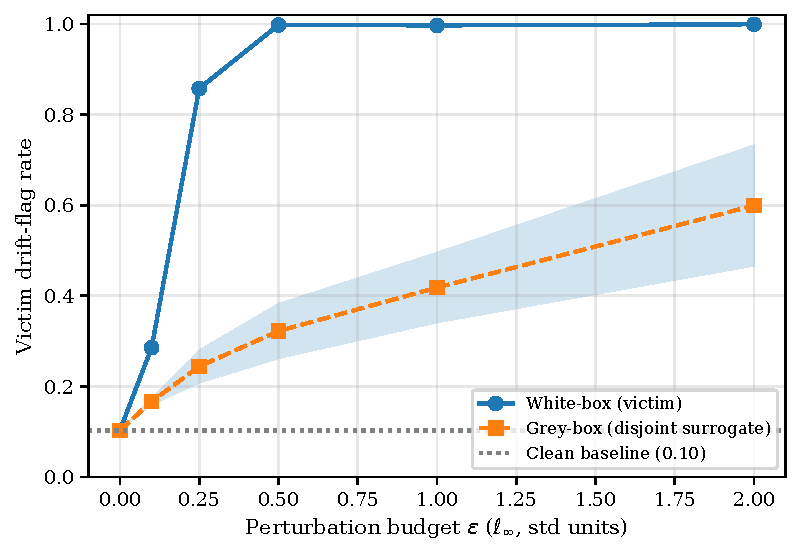
\includegraphics[width=0.7\linewidth]{../experiments/contrastive_ncm/figures/rq3_pgd_false_positive.pdf}
    \caption{PGD false-positive attack on per-sample detection: fraction of perturbed known-class flows the victim flags as drifted versus the $L_\infty$ budget, white-box against the victim and grey-box via surrogate transfer.}
    \label{fig:eval-rq3-pgd}
\end{figure}

\subsection{Forcing the Concept Trigger}
\label{sec:eval-rq3-force}
Forcing therefore requires displacing the batch mean coherently. Naively applying coherent perturbations along a random direction fails. Even white-box at $\epsilon = 2.0$ the accumulated displacement reaches only $29.5$, short of the required threshold $T = 39.3$, and forces no fire. This is what initially looked like robustness. However, we conclude that it is not; it is a weak attack. An aimed mean-shift attack, which optimises two opposing perturbations to maximise the separation of the encoder's batch means, crosses $T$ at $\epsilon \ge 1.0$, reaching displacements of $47$ at $\epsilon = 1.0$ and $92$ at $\epsilon = 2.0$ (\cref{tab:rq3-pgd-meanshift}). Thereby forcing a concept-discovery event white-box.

\begin{table}
\caption{Accumulator attack via direct latent mean-shift: PGD jointly optimises two pools to maximise the separation of their drifted-batch means (the quantity the concept-discovery accumulator integrates), rather than pushing along a fixed random direction. A fire is forced only if the displacement exceeds $T$.}
\label{tab:rq3-pgd-meanshift}
\centering
\begin{tabular}{lccccr}
\toprule
 & Flag A & Flag B & Displacement & Threshold ($T$) & Forces fire? \\
$L_\infty$ budget ($\epsilon$) &  &  &  &  &  \\
\midrule
0.10 & 0.23 & 0.11 & 18.0 & 39.3 & False \\
0.25 & 0.75 & 0.17 & 26.1 & 39.3 & False \\
0.50 & 0.77 & 0.86 & 25.6 & 39.3 & False \\
1.00 & 1.00 & 1.00 & 47.1 & 39.3 & True \\
2.00 & 1.00 & 1.00 & 91.5 & 39.3 & True \\
\bottomrule
\end{tabular}
\end{table}


The most consequential result is that this attack transfers. Crafted against a data-disjoint surrogate and evaluated on the victim, the mean-shift retains roughly $70\%$ of its white-box displacement -- $33$ at $\epsilon = 1.0$ and $65$ at $\epsilon = 2.0$ (\cref{tab:rq3-pgd-meanshift-greybox}). That clears $T = 39.3$ and forces a fire at $\epsilon = 2.0$ while at $\epsilon = 1.0$ the transferred displacement falls just short. This stands in sharp contrast to per-sample detection, which transferred poorly ($\le 60\%$): a per-sample flag requires every sample to individually clear the threshold, which is brittle across two independently-trained encoders. Whereas, the trigger fires on a batch mean and averaging launders the per-sample transfer noise, leaving the coherent direction both encoders agree on. The batch-mean statistic the detector adopts for stability is precisely what makes the trigger grey-box forceable.

\begin{table}
\caption{Grey-box mean-shift transfer. Two pools are optimised against a disjoint surrogate (trained on a held-out 40 percent of the known-class pool, with no flows shared with the victim) and the displacement of their drifted-batch means is measured on the victim. Reported are the mean and std of the transferred displacement over three surrogate seeds and the number of seeds whose transfer forces a victim concept-discovery fire. A fire requires the displacement to exceed $T$ (compare the white-box mean-shift,~\cref{tab:rq3-pgd-meanshift}).}
\label{tab:rq3-pgd-meanshift-greybox}
\centering
\begin{tabular}{lrrr}
\toprule
 & Displacement & Threshold ($T$) & Seeds forcing fire \\
$L_\infty$ budget ($\epsilon$) &  &  &  \\
\midrule
0.10 & 11.1 $\pm$ 0.7 & 39.3 & 0/3 \\
0.25 & 18.3 $\pm$ 1.1 & 39.3 & 0/3 \\
0.50 & 20.7 $\pm$ 1.6 & 39.3 & 0/3 \\
1.00 & 33.1 $\pm$ 2.0 & 39.3 & 0/3 \\
2.00 & 65.0 $\pm$ 3.8 & 39.3 & 3/3 \\
\bottomrule
\end{tabular}
\end{table}


The caveat is the budget. Grey-box forcing requires $\epsilon = 2.0$ here, a large, unconstrained $L_\infty$ perturbation in standardised-feature units that would almost certainly distort flows beyond what protocol constraints permit; a feature-constrained mean-shift would raise the bar further and is left to future work. Within the adopted grey-box threat model, however, the conclusion stands: the concept trigger is forceable, not robust, and the attack is bounded only by the perturbation budget.

\subsection{Decomposing the Firing Gate}
\label{sec:eval-rq3-gate}
The firing predicate is made up of three conjuncts -- displacement, count, and fraction (\cref{sec:axt-surface}). To attribute the system's behaviour to the individual floors we ablate the count and fraction conditions independently, across \texttt{displacement-only} (the paper's rule, neither floor), \texttt{count-only}, \texttt{fraction-only}, and the \texttt{full} gate we propose.

\begin{table}
\caption{Gate ablation (forcing): pre-drift injection of true-labelled novel flows under the four decomposed firing gates of the count/fraction 2x2. Values reported are mean $\pm$ std over seeds.}
\label{tab:rq3-gate-forcing}
\centering
\begin{tabular}{llr}
\toprule
 &  & Forced fires \\
Gate & Poison \% &  \\
\midrule
\multirow[t]{4}{*}{Displacement-only} & 2\% & 0.667 $\pm$ 0.943 \\
 & 5\% & 14.667 $\pm$ 2.867 \\
 & 10\% & 5.000 $\pm$ 2.160 \\
 & 20\% & 0.000 $\pm$ 0.000 \\
\cline{1-3}
\multirow[t]{4}{*}{Count-only} & 2\% & 0.333 $\pm$ 0.471 \\
 & 5\% & 1.667 $\pm$ 0.943 \\
 & 10\% & 2.333 $\pm$ 0.943 \\
 & 20\% & 0.000 $\pm$ 0.000 \\
\cline{1-3}
\multirow[t]{4}{*}{Fraction-only} & 2\% & 0.000 $\pm$ 0.000 \\
 & 5\% & 0.000 $\pm$ 0.000 \\
 & 10\% & 0.000 $\pm$ 0.000 \\
 & 20\% & 0.000 $\pm$ 0.000 \\
\cline{1-3}
\multirow[t]{4}{*}{Full} & 2\% & 0.000 $\pm$ 0.000 \\
 & 5\% & 0.000 $\pm$ 0.000 \\
 & 10\% & 0.000 $\pm$ 0.000 \\
 & 20\% & 0.000 $\pm$ 0.000 \\
\bottomrule
\end{tabular}
\end{table}


\begin{table}
\caption{Gate ablation (suppression): benign-labelled injection at p=25\% during genuine drift under the four decomposed firing gates of the count/fraction 2x2. Reported values are the mean $\pm$ std over seeds.}
\label{tab:rq3-gate-suppression}
\centering
\begin{tabular}{lrr}
\toprule
 & Fri $F_1$ & Retrains \\
Gate &  &  \\
\midrule
Displacement-only & 0.620 $\pm$ 0.036 & 134.667 $\pm$ 22.366 \\
Count-only & 0.207 $\pm$ 0.000 & 0.000 $\pm$ 0.000 \\
Fraction-only & 0.207 $\pm$ 0.000 & 0.000 $\pm$ 0.000 \\
Full & 0.207 $\pm$ 0.000 & 0.000 $\pm$ 0.000 \\
\bottomrule
\end{tabular}
\end{table}


Against forcing (\cref{tab:rq3-gate-forcing}, pre-drift injection of true-labelled flows), the two floors are not equal. The fraction floor alone blocks every forced fire at every budget, because at low injection the attacker's flows are only a small fraction of the drifted buffer which is already padded by the detector's own false positives, so the $0.3$ threshold is never reached. The count floor reduces the efficacy of forcing. It cuts forced fires from $14.7$ to $1.7$ at $p = 5\%$, but it alone is not sufficient since the $500$ samples it demands are within a determined attacker's budget. The full gate, exactly like fraction-only, is completely immune.

Against suppression (\cref{tab:rq3-gate-suppression}, benign injection at $p = 25\%$), the picture inverts. Either floor alone suffices to make the system suppressible. The \texttt{count-only}, \texttt{fraction-only}, and \texttt{full} gates all collapse to the no-adaptation floor ($F_1 = 0.207$, zero retrains), while only \texttt{displacement-only} keeps adapting. However, it does so pathologically, firing approximately $135$ times on the injected noise, and is in turn the most forceable gate of all. The only configuration we examine that resists suppression is the one that cannot resist forcing.

The ablation demonstrates the trade-off of this trigger-gated adaptation mechanism. The suppression vector is over-determined. Any floor placed on the buffer's makeup to resist forcing or premature firing simultaneously hands the adversary a way to hold the buffer below it and starve adaptation. The two floors are defeated by different mechanisms -- the fraction floor by direct dilution (benign flows drive the attack fraction below $0.3$), the count floor is more subtle. Because the displacement accumulator is only reset when the trigger is fired (\cref{eq:concept-accumulator}), a gate that withholds firing lets it telescope into a stationary regime in which $\|\Delta\|$ stays below $T$ even after the count is satisfied. Resetting or windowing the accumulator on gated crossings could be implemented as mitigations, but we leave this to future work. The design implication is stark: under makeup-based gating, making the trigger harder to force and harder to suppress are in direct tension.

\section{Summary}
\label{sec:eval-summary}
The three research questions resolve as follows. RQ1: the trigger-dependent coupling exposes a trigger channel and a composition channel that gate all adaptation, and both are invisible to the detector-only evaluation the literature uses. RQ2: the composition channel \emph{resists} boundary poisoning but it does \emph{not} resist a backdoor, which installs a trigger-activated shortcut beside the clean boundary and persists through the exemplar memory; the same channel also decides whether $\mathcal{M}$ adapts at all (the $p = 25\%$ suppression collapse), compounded by a structural blind spot in which the detector never discovers \texttt{PortScan}. RQ3: the firing trigger is forceable, not robust. An aimed mean-shift attack forces a concept-discovery event both white-box and grey-box (retaining roughly $70\%$ of its displacement against a data-disjoint surrogate); and the gate ablation shows the two firing floors are over-determined, so any floor that resists forcing simultaneously enables suppression. Across all three, the throughline is that coupling a robust detector to a base learner does not make the system robust: the security is further decided at the coupling, a conclusion~\cref{ch:conclusion} draws together.

% We note for completeness that a \emph{flipped-label} manufactured-novelty payload --- attack flows presented under a wrong novel label --- is blocked by the fraction floor at every budget, so an attacker cannot register an arbitrary spurious concept on demand. The complementary \emph{durable}-poison case of~\cref{sec:axt-maintenance} --- poisoning at a damaging rate then running clean, so the payload persists via the never-evict exemplar memory --- is examined directly for the composition channel in~\cref{sec:eval-rq2}.
